\chapter{Analisis}
\label{chap:analisis}
Bab ini berisi analisis BPMN dengan menggunakan skenario, analisis \textit{event} yang terkait dengan integrasi sistem email, dan mekanisme integrasi sistem email.
\section{Analisis BPMN}
\label{sec:analisisbpmn}

\subsection{Skenario Proposal Bisnis}
\label{skenario1}
John mempunyai ide proposal bisnis untuk manajernya, Peter. John menulis dan mengunggah proposal melalui sistem Camunda. Sebelum proposal disetujui, Peter harus memeriksa apakah proposalnya layak atau tidak. Jika proposalnya tidak layak, John harus memperbaiki dan mengunggahnya kembali. \textit{Workflow} dari skenario ini sebagai berikut :
		\begin{figure}[H]
			\centering
			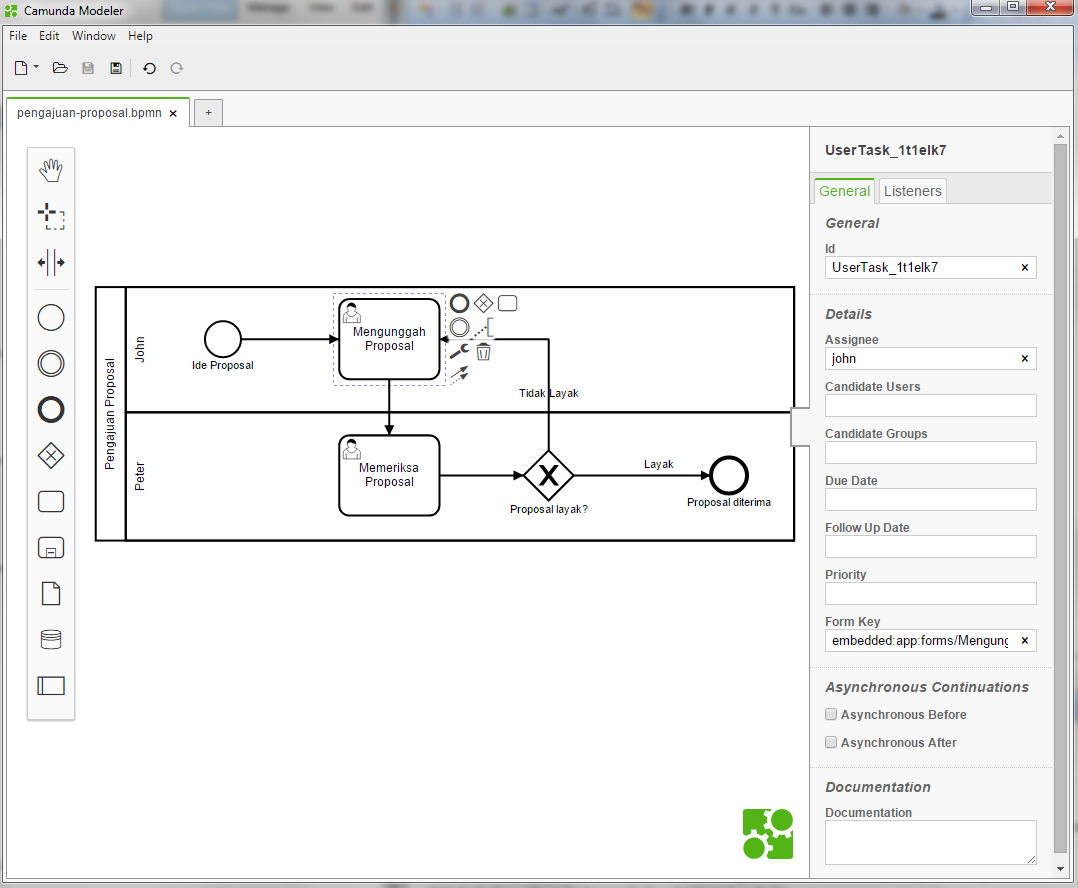
\includegraphics[scale=0.5]{Gambar/Bab-3/Kasus1-2}
			\caption{Mengunggah Proposal} 
			\label{fig:mengunggahproposal}
		\end{figure}
		
Pada Gambar ~\ref{fig:mengunggahproposal}, terdapat beberapa atribut yang memiliki nilai, yaitu :
\begin{itemize}
	\item Id, yaitu id dari \textit{task} yang dipilih
	\item Assignee, yaitu aktor yang akan mengerjakan \textit{task}
	\item Form Key, yaitu tautan ke file HTML yang berupa tampilan untuk mengunggah proposal.
\end{itemize}

\subsection{Skenario Proposal Bisnis dari Group}
\label{skenario2}
Pegawai di perusahaan X memiliki tiga divisi yaitu \textit{accounting}, \textit{sales}, dan \textit{management}. Divisi \textit{accounting} dan \textit{sales} dapat mengajukan proposal bisnis ke divisi \textit{management}. Sama seperti Skenario~\ref{skenario1}, divisi \textit{management} harus memeriksa apakah proposalnya layak atau tidak. Jika proposalnya tidak layak, pembuat proposal harus memperbaiki dan mengunggahnya kembali. Workflow dari skenario ini sebagai berikut :

		\begin{figure}[H]
			\centering
			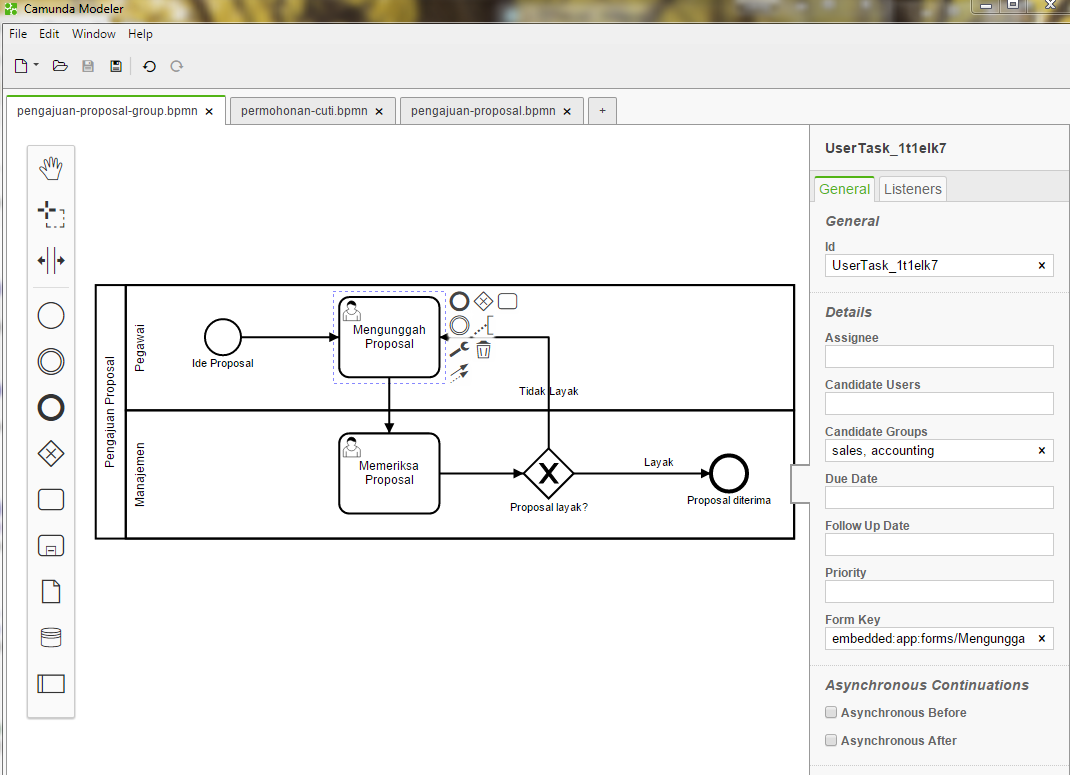
\includegraphics[scale=0.5]{Gambar/Bab-3/Kasus2-1}
			\caption{Mengunggah Proposal} 
			\label{fig:mengunggahproposalgroup}
		\end{figure}
Pada Gambar ~\ref{fig:mengunggahproposalgroup}, terdapat atribut \textit{Candidate Groups}. Atribut ini melambangkan bahwa \textit{task} ini dapat dikerjakan oleh salah satu anggota dari grup \textit{accounting} atau grup \textit{sales}.


\section{\textit{Event} yang Terkait dengan Integrasi Sistem Email}
\label{sec:eventUserTask}

Integrasi Camunda dengan sistem email pada skripsi ini bertujuan untuk memberi tahu aktor Camunda apabila ada \textit{tasks} yang perlu dikerjakan oleh aktor. Ketika aktor menerima email mengenai \textit{tasks} yang perlu dikejakan, aktor dapat langsung mengerjakannya. 

Camunda memiliki berbagai jenis \textit{tasks} seperti \textit{user tasks, manual tasks, service task}, dan lainnya. Karena proses integrasi email dengan Camunda melibatkan aktor (aktor menerima pemberitahuan pekerjaannya melalui email), \textit{task} yang akan diintegrasikan dengan sistem email adalah \textit{user tasks}.

\section{Mekanisme Integrasi Sistem Email}
\label{integrasi}
\textit{User tasks} memiliki atribut \textit{Task Listener} yang dapat mengeksekusi perintah. \textit{Task Listener} memiliki dua atribut, yaitu \textit{Event Type} dan \textit{Listener Type}. Terdapat empat pilihan dari \textit{Event Type}, yaitu \textit{create, assignment, complete, delete}. 
		\begin{figure}[H]
			\centering
			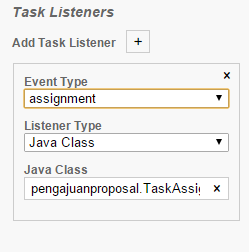
\includegraphics[scale=1]{Gambar/Bab-3/TaskListener}
			\caption{Event Task Listener} 
			\label{fig:eventtasklistener}
		\end{figure}
\begin{itemize}
	\item Create, perintah dieksekusi ketika \textit{task} telah dibuat dan siap untuk dikerjakan. 
	\item Assignment, perintah dieksekusi ketika aktor yang akan mengerjakan \textit{task} sudah ditentukan.
	\item Complete, perintah dieksekusi ketika \textit{task} sudah dikerjakan dan sebelum \textit{task} dihapus.
	\item Delete, perintah dieksekusi setelah \textit{task} dihapus.
\end{itemize}


Untuk mengintegrasikan \textit{user tasks} dengan email, \textit{event type} yang dapat digunakan adalah \textit{create} dan \textit{assignment}. \textit{Event complete} dan \textit{delete} tidak dapat digunakan untuk memberi tahu aktor karena setelah \textit{task} selesai dan dihapus, alamat email untuk \textit{Task} selanjutnya belum diambil sementara \textit{event} sudah selesai dipanggil.

Apabila menggunakan \textit{event create}, \textit{task} harus memiliki pemiliknya masing-masing ketika BPMN dibuat atau memiliki \textit{candidate user/group}. Bila pemilik \textit{task} belum ditentukan, email tidak akan terkirim, karena \textit{event create} sudah selesai dipanggil sebelum \textit{task} memiliki pemilik. Pengiriman email untuk \textit{task} yang belum memiliki aktor dapat menggunakan \textit{event create}. Sedangkan pada \textit{event assignment}, pengiriman email dilakukan setelah \textit{task} didelegasikan ke masing-masing user.




